\begin{filecontents*}{\jobname.xmpdata}
  \Title{Building a Ray-Traced Rendering Engine on Sparse Voxel Grids}
  \Author{10834225}
  \Language{en-GB}
  \Copyrighted{True}
\end{filecontents*}

\documentclass{extra}

%%%%%%%%%%%%%%%%%% PACKAGES AND COMMANDS %%%%%%%%%%%%%%%%%%
\usepackage{graphicx,psfrag,color} % for postscript graphics files
  \graphicspath{ {./figures/} }
\usepackage{amsmath}               % assumes amsmath package installed
  \allowdisplaybreaks[1]           % allow eqnarrays to break across pages
\usepackage{amssymb}               % assumes amsmath package installed
\usepackage{url}                   % format hyperlinks correctly
\usepackage{rotating}              % allow portrait figures and tables
\usepackage{multirow}              % allows merging of rows in tables
\usepackage{lscape}                % allows pages to be typeset in landscape mode
\usepackage{tabularx}              % allows fixed width tables
\usepackage{verbatim}              % enhanced version of built-in verbatim environment
\usepackage{footnote}              % allows more control over footnote environments
\usepackage{float}                 % allows H option on floats to force here placement
\usepackage{booktabs}              % improve table line spacing
\usepackage{lipsum}                % for adding dummy text here
\usepackage[base]{babel}           % for proper hypthenation in lipsum sections
\usepackage{subcaption}            % for multiple sub-figures in a single float
\usepackage{cleveref}
\usepackage{xcolor}
\usepackage{color}
\usepackage[inkscapelatex=false]{svg}
\usepackage[acronym]{glossaries}
\usepackage{listings}
\usepackage{listings-rust}
\usepackage{multicol}
\usepackage{bm}
\usepackage{enumitem}
\newtheorem{theorem}{Theorem}
\newcommand{\degree}{\ensuremath{^\circ}}
\newcommand{\sus}[1]{$^{\mbox{\scriptsize #1}}$} % superscript in text (e.g. 1st)
\newcommand{\sub}[1]{$_{\mbox{\scriptsize #1}}$} % subscript in text
\AtBeginEnvironment{quote}{\par\singlespacing\small}

%%%%%%%%%%%%%%%%%% REFERENCES SETUP %%%%%%%%%%%%%%%%%%
\usepackage[style=ieee,backend=biber,backref=true,hyperref=auto,backend=bibtex]{biblatex}
% \DefineBibliographyStrings{english}{backrefpage = {cited on p\adddot},  backrefpages = {cited on pp\adddot}}
\addbibresource{ref.bib}

\makeglossary
\newacronym{gcd}{GCD}{Greatest Common Divisor}

%%%%%%%%%%%%%%%%%% START DOCUMENT %%%%%%%%%%%%%%%%%%
\begin{document}
\makeatletter
\title{\xmp@Title}
\studentid{\xmp@Author}
\makeatother

\course{Computer Science}
\submitdate{2024}
\wordcount{many}
\maketitle



%%%%%%%%%%%%%%%%%% LISTS OF CONTENT %%%%%%%%%%%%%%%%%%
\uomtoc
% other lists are not required, but can include \uomlof and \uomlot if really want to

\uomlof

\uomlot

%%%%%%%%%%%%%%%%%% ABSTRACT %%%%%%%%%%%%%%%%%%
\begin{abstract} % put abstract here. Limit is 1 page.
Rendering engines are critical in computer graphics, serving as the backbone of visualisation for digital media, including video games, simulations, virtual reality, and animated films. These engines are responsible for converting 3D models, textures, and lighting information into the compelling images users see on their screens. A rendering engine's efficiency and capabilities directly influence the digital experience's realism and interactivity.

This thesis explores the development and implementation of a ray-traced voxel rendering engine utilising sparse grids to enhance real-time rendering capabilities. The focus is on leveraging sparse data structures to manage volumetric data efficiently, thus allowing for intricate rendering details and high performance. The research investigates various techniques in ray tracing to optimise the rendering process. The outcomes demonstrate that sparse voxel grids combined with discrete signed distance fields can significantly reduce memory usage while maintaining rendering speed. This work contributes to computer graphics and game development by providing insights into the application of sparse data structures in real-time rendering environments.
\end{abstract}%
\clearpage


%%%%%%%%%%%%%%%%%% DECLARATIONS %%%%%%%%%%%%%%%%%%
\uomdeclarations % Don't need unless final thesis


\begin{uomacknowledgements}
  I would like to express my gratitude to my supervisor, Prof. Steve Pettifer, for his guidance, encouragement, and expertise throughout this research project. My thanks also go to my partner Diana, whose support and understanding have been my anchor in my academic pursuits. I also extend my deepest appreciation to my parents, whose love and belief in my potential have been my constant motivation.
\end{uomacknowledgements}

%%%%%%%%%%%%%%%%%% CONTENT %%%%%%%%%%%%%%%%%%
%%% Local Variables:
%%% mode: latex
%%% TeX-master: "../main"
%%% End:

\part{Introduction}
\section{Motivation}
\section{Aims}
\section{Objectives}
\section{Report structure}

%%% Local Variables:
%%% mode: latex
%%% TeX-master: "../main"
%%% End:

\part{Background and Literature Review}\label{backgorund}
\section{Rendering engines}
Graphics engines are the core software components responsible for rendering visual content in applications ranging from video games to scientific simulations and movie visual effects.
Engines abstract the complexities of rendering by providing developers with high-level tools and interfaces to represent digital environments.

Rendering engines have evolved from the simple wire-frame models of the 1960s to today's complex 3D systems, driven by advancements in computational power and graphical standards\cite{old} like OpenGL introduced in the early 1990s.

\subsection{Primitves}
At the heart of any graphical engine is the concept of primitives, the simplest forms of graphical objects that the engine can process and render. Primitives are building blocks from which more complex shapes and scenes can be constructed.

\textbf{Polygons}, particularly triangles, are the most commonly used primitives in 3D graphics. This is owed to their simplicity and flexibility, allowing the construction of virtually any 3D shape through \emph{tesselation}. Polygonal meshes define the surfaces of objects in a scene, with each polygon vertex typically associated with additional information such as colour, texture coordinates, and normal vectors for lighting calculations.

\textbf{Voxels} represent a different approach to defining 3D shapes; they are essentially three-dimensional pixels. Where polygons define surfaces, voxels establish volume, with each voxel potentially containing colour and density information.
This characteristic makes voxels particularly well-suited for rendering scenes with materials that have intricate internal structures, such as fog, smoke, fire, and fluids.

\subsection{Ray-tracing vs. Rasterization}
Rendering engines can utilise two main rendering techniques for rendering scenes: ray tracing and rasterisation. Both have advantages and trade-offs.

\textbf{Rasterization} is the most widespread technique used in real-time applications.
It converts the 3D scene into a 2D image by projecting vertices onto the screen, filling in pixels that makeup polygons, and applying textures and lighting.
Over the development of the graphics programming industry, graphics hardware has become extremely efficient at performing rasterisation, making it the standard for video games and interactive applications.

\textbf{Ray-Tracing}, in contrast, simulates the path of light as rays travelling through a scene to produce images with realistic lighting, shadows, reflections, and refractions. Ray tracing is computationally intensive but yields higher-quality images, making it favoured for applications where visual fidelity is critical. However, recent advancements in hardware have begun to bring real-time ray tracing to interactive applications.

Ray tracing, conceptualised by Arthur Appel in 1968\supercite{appel}, offers photorealistic images by simulating light paths, but its computational intensity limited early use to non-real-time applications. Rasterisation, popularised in the 1970s and optimised by GPU advancements, became the standard for real-time graphics, though \emph{recent} hardware innovations are now enabling real-time ray tracing.

\section{Representing voxels}
Various data structures can be employed to represent and manipulate voxels in program memory efficiently. Each method entails trade-offs between memory usage, access speed, and implementation complexity. Access speed refers to the time complexity of querying the data structure at an arbitrary point in space to retrieve a potential voxel.

\subsection{Voxel grids}
A voxel grid is the most straightforward and intuitive approach to representing volumetric data. The 3D space is divided into a regular grid of voxels, each holding information such as colour, material properties, or density. This method provides direct $O(1)$ access to voxel data.

However, this simplicity comes at a significant disadvantage: memory consumption.
As the bounding volume or the level of detail of the scene increases, the memory required to store the voxel grows by $O(N^{3})$.
Additionally, empty space can occupy a majority of the memory space.
For example, consider a scene with two voxels a million units apart in all axes.
A voxel grid would have to store all the empty voxels in-between; $10^{18}$ memory units reserved, 2 of which carry useful data.
This limitation makes the naive voxel grids impractical for large or highly detailed scenes.

\subsection{Hierarchical voxel grids (N-trees)}
Hierarchical grids, such as octrees, are employed to mitigate these issues. An octree is a tree data structure where each node represents a cubic portion of 3D space and has up to eight children. This division continues recursively, allowing for varying levels of detail within the scene: larger volumes are represented by higher-level nodes, while finer details are captured in lower levels.

The primary advantage of using an octree is spatial efficiency. Regions of the space that are empty or contain uniform data can be represented by a single node, significantly reducing the memory footprint. Furthermore, octrees facilitate efficient querying operations, such as collision detection and ray tracing, by allowing the algorithm to discard large empty or irrelevant regions of space quickly.

Hierarchical grids introduce complexity in terms of implementation and management. Operations such as updating the structure or balancing the tree to ensure efficient access can be more challenging than those of uniform grids.
Another sacrifice is access time, as querying an arbitrary region of space can entail walking down the tree for several levels.
Nonetheless, the benefits of hierarchical representations often outweigh these drawbacks for applications requiring large, detailed scenes with a mix of dense and sparse regions. Therefore, N-trees are frequently used in voxel engines.

Donald Meagher introduced the concept of octrees in 1980\supercite{donald} as a means to manage spatial data in 3D computer graphics efficiently. This technique quickly became integral in applications like 3D rendering and geometric modelling, where it revolutionized spatial data optimization by balancing detailed representation with computational efficiency.

\subsection{VDB}
\newacronym{bpt}{B+tree}{A m-ary tree with a variable but often large number of children per node.}
\newacronym{vdb}{VDB}{Volumetric Dynamic B+tree grid data structure introduced by Ken Museth\supercite{vdb2013}}

\textbf{\acrshort{vdb}} was introduced in 2013 by Ken Museth\supercite{vdb2013} from the DreamWorks Animation team.
\begin{quote}
It is a Volumetric, Dynamic grid that shares several characteristics with B+trees.
It exploits spatial coherency of time-varying data to separately and compactly encode data values and grid topology.
VDB models a virtually infinite 3D index space that allows for cache-coherent and fast data access into sparse volumes of high resolution.
\end{quote}

At its core, VDB functions as a shallow N-tree with a fixed depth, where nodes at different levels vary in size. The top level of this tree structure is managed through a hash map, enabling VDB models to cover extensive index spaces with minimal memory overhead. This design achieves $O(1)$ access performance and effectively stores tiled data across vast spatial regions.

The VDB data structure was introduced along with several algorithms that fully use the data structure's features, offering significant improvements in techniques for efficiently rendering volumetric data. These are some of VDB's benefits, as detailed in the original paper.
\begin{enumerate}
  \item \emph{Dynamic}. Unlike most sparse volumetric data structures, VDB is developed for both dynamic topology and dynamic values typical of time-dependent numerical simulations and animated volumes.
  \item \emph{Memory effcient}. The dynamic and hierarchical allocation of compact nodes leads to a memory-efficient sparse data structure that allows for extreme grid resolution.
  \item \emph{Fast random and sequential data access}. VDB supports fast, constant-time random data lookup, insertion, and deletion.
  \item \emph{Virtually infinite}. VDB, in concept, models an unbounded grid in the sense that the accessible coordinate space is only limited by the bit-precision of the signed coordinates.
  \item \emph{Efficient hierarchical algorithms.} The \acrshort{bpt} structure offers the benefits of cache coherency, inherent bounding-volume acceleration, and fast per-branch (versus per-voxel) operations.
\end{enumerate}
These benefits make VDB a very compelling data structure that serves as the building block of a voxel-based rendering engine.

\section{Ray tracing}
To render a scene using ray tracing, camera rays are shot through the view frustum and into the scene. At each object intersection, part of a ray is absorbed, reflected, and refracted. To achieve realistic results, a rendering engine needs to model as many of these light interactions as possible in each frame's time budget.

This section delves into integrating ray tracing within the graphics pipeline and the methods used to implement it, focusing on casting a ray through a scene.

\subsection{Graphics pipeline}
The graphics pipeline of a rendering engine is the underlying system of a rendering engine that transforms a 3D scene into a 2D representation that is then presented on a screen. While rasterization transforms 3D objects into 2D images through a series of stages(vertex processing, shape assembly, geometry shading, rasterization, and fragment processing), the ray tracing pipelines introduce a paradigm shift. It primarily involves calculating the path of rays from the eye (camera) through pixels in an image plane and into the scene, potentially bouncing off surfaces or passing through transparent materials before contributing to the colour of a pixel.

Calculating a ray's path is central to ray tracing, so the performance of the algorithm that does this calculation is critical.
\subsection{Casting a ray}
Ray casting techniques vary depending on the representation of the 3D world within the rendering engine.
This section introduces basic ray casting techniques, while subsequent discussions cover methods specific to voxel-based environments.

\vspace{0.5cm}
\textbf{Ray marching}

A straightforward way to represent a 3D environment would be a mathematical function of sorts.
It would take the coordinates of a point as input and return the material's properties at that point (provided an object is present).

The first algorithm one might develop when trying to cast a ray through an unknown scene is ray marching.
It involves incrementally stepping along a ray, sampling the scene for collisions at each step.
The chosen step size must be sufficiently small to ensure no detail is missed.

While simple, ray marching has drawbacks, especially in terms of performance.
Considering the need to process millions of pixels per frame within the time constraints of high frame rates, it becomes apparent that iterating a ray tens of thousands of times for every pixel is impractical for modern engines.

These constraints require exploring more advanced techniques to meet the goal of visual realism and performance.

\vspace{0.5cm}
\textbf{Ray casting}

A 3D environment could also be represented as a collection of polygons that form meshes.

Ray casting finds the intersection of rays with geometric primitives (e.g. triangles and circles). This method skips stepping along the ray entirely by using the underlying mathematics of intersecting lines with polygons.

The fundamental issue with this approach is that rays must be checked for an intersection with all the primitives in the scene. Thus, computing a single ray's intersection has linear complexity in terms of the number of polygons in the scene.


\vspace{0.5cm}
\phantomsection\label{def:sdf}
\textbf{SDF}
\newacronym{sdf}{SDF}{Signed distance fields, described in \cref{def:sdf}}

Signed distance fields (\acrshort{sdf}) are a different way of representing the environment. An SDF provides the minimum distance from a point in space to the closest surface, allowing the ray marching algorithm to skip empty space and efficiently determine surface intersections.
With the distance to the nearest surface known, ray marching can be performed by stepping along the ray with that distance, drastically reducing the number of steps needed to cast a ray.

Combining SDF with ray marching offers a powerful method for rendering complex scenes, including soft shadows, ambient occlusion, and volumetric effects.
This combination is highly flexible and can create highly detailed and intricate visual effects, particularly in procedural rendering and visual effects.

SDFs are not without drawbacks. They can be difficult to maintain and computationally expensive to generate or update. In practice, distance data cannot be of arbitrary size, as that distance information comes at the cost of program memory.

SDFs have been used in real-time rendering, usually in a raymarching context, starting in the mid-2000s. In 2007, Valve used SDFs to render large pixel-size smooth fonts on the GPU in its games\supercite{valve}.

\subsection{Casting a ray on a voxel grid}
The ray casting methods presented so far do not take advantage of the discrete voxel grid on which this rendering engine is based. This section presents efficient algorithms that can use the underlying representation of a hierarchical voxel grid.

\vspace{0.5cm}
\phantomsection\label{def:dda}
\textbf{DDA}
\newacronym{dda}{DDA}{Digital Differential Analyzer, line drawing algorithm described in \cref{def:dda}}

Basic ray marching can be improved on a discrete voxel grid by stepping from voxel to voxel. Because voxels are the smallest unit of space, a ray can safely step from one to the next, ensuring there is nothing else in between.

The Digital Differential Analyzer (\acrshort{dda}) line drawing algorithm does precisely that; it marches along a ray from voxel to voxel, skipping all space in between.

DDA works by breaking down the minimum distance a ray travels to intersect a grid line on each axis.
At each iteration, it steps to the closest grid intersection along the ray.

\vspace{0.5cm}
\phantomsection\label{def:hdda}
\newacronym{hdda}{HDDA}{Hierarchical \acrshort{dda}, line drawing algorithm described in \cref{def:hdda}}
\textbf{HDDA}

On a hierarchical grid, the DDA algorithm can take advantage of the data structure's topology by stepping through empty, larger chunks.
A ray cast using \acrshort{hdda} essentially performs DDA at the level in the tree it is currently at.

Ken Museth introduced a version of the HDDA algorithm for the VDB data structure in 2014\supercite{vdb2014}.
This algorithm can be highly efficient; large empty areas can be skipped in a single step, drastically reducing the required steps to march a ray.

\section{Summary of similar systems}
\subsection{OpenVDB\supercite{openvdb:doc}}

\begin{quote}
``OpenVDB is an Academy Award-winning open-source C++ library comprising a novel hierarchical data structure and a suite of tools for the efficient storage and manipulation of sparse volumetric data discretized on three-dimensional grids. It was developed by DreamWorks Animation for use in volumetric applications typically encountered in feature film production and is now maintained by the Academy Software Foundation (ASWF).
''
\end{quote}

This voxel rendering engine is made on the same backend as this project, Rust and wgpu. However, it employs a more standard approach to rendering, generating triangle meshes from voxel data and performing rasterization.

\subsection{All is Cubes\supercite{cubes}}

\begin{quote}
``This project is a game engine for worlds made of cubical blocks (“blocky voxels”). The particular features of this engine are that each ordinary block is itself made out of blocks, and all game mechanics are defined by data within the world that can be interactively edited.''
\end{quote}

This is a voxel rendering engine made on the same backend as this project, Rust and wgpu, however it employs a more standard apprach of rendering, generating triangle meshes from voxel data and performing rasterization.

\subsection{ Unique Contribution of this Project}
To the best of my knowledge, there is currently no fully operational voxel rendering engine built solely on the VDB data structure. This project aims to fill that gap by developing a comprehensive rendering engine based entirely on VDB, leveraging its capabilities to efficiently handle complex and detailed volumetric data. Unlike other systems, which may integrate VDB as one of many components or use it for specific functions, this engine is designed to utilize VDB as the core framework for all rendering tasks. This distinction sets the project apart, offering a new perspective and opportunities to explore novel ray-tracing techniques.

%%% Local Variables:
%%% mode: latex
%%% TeX-master: "../main"
%%% End:

\section{Methodology}
This section outlines the implementation details of the voxel rendering engine, starting from the selection of programming languages and libraries, going over the architecture of the engine, and diving deep into the data structures and algorithms employed, particularly focusing on VDB for voxel representation and the optimization of ray casting algorithms.
Finally, this section will discuss the extension of these algorithms to full-fledged ray tracing, allowing for dynamic lightning and glossy material support.

\subsection{Rust \& Wgpu}
\hyphenation{WebGPU}

The voxel rendering engine is built using \textbf{Rust}, a programming language known for its focus on safety, speed, and concurrency\supercite{rustbook}.
Rust's design emphasizes memory safety without sacrificing performance, making it an excellent choice for high-performance applications like a rendering engine.
The language's powerful type system and ownership model prevent a wide class of bugs, making it ideal for managing the complex data structures and concurrency challenges inherent in rendering engines. Thanks to this no memory leak or null pointer was ever encoutered throughout the developmenent of this project.

For the graphical backend, the engine utilizes \textbf{wgpu}\supercite{wgpu}, a Rust library that serves as a safe and portable graphics API. wgpu is designed to run on top of various backends, including Vulkan, Metal, DirectX 12, and WebGL, ensuring cross-platform compatibility. This API provides a modern, low-level interface for GPU programming, allowing for fine-grained control over graphics and compute operations. wgpu is aligned with the WebGPU specification\supercite{webgpu:doc}, aiming for broad support across both native and web platforms.
This choice ensures that the engine can leverage the latest advancements in graphics technology while maintaining portability and performance.

The combination of Rust and wgpu offers several advantages for the development of a rendering engine:

\begin{enumerate}
  \item \emph{Safety and Performance:} Rust’s focus on safety, coupled with wgpu's design, minimizes the risk of memory leaks and undefined behaviors, common issues in high-performance graphics programming. This is thanks to Rust's idea of zero-cost abstractions.

  \item \emph{Cross-Platform Compatibility:} With wgpu, the engine is not tied to a specific platform or graphics API, enhancing its usability across different operating systems and devices.

  \item \emph{Future-Proofing:} wgpu's adherence to the WebGPU specification ensures that the engine is built on a forward-looking graphics API, designed to be efficient, powerful, and broadly supported. It also allows the future option of supporting web platforms, once browsers adopt WebGPU more throughly.

  \item \emph{Concurrency:} Rust’s advanced concurrency features enable the engine to efficiently utilize multi-core processors, crucial for the heavy computational demands of rendering pipelines.
\end{enumerate}

These technical choices form the foundation upon which the voxel rendering engine is constructed. Following this, the engine's architecture is designed to take full advantage of Rust's performance and safety features and wgpu's flexible, low-level graphics capabilities, setting the stage for the implementation of advanced voxel representation techniques and optimized ray tracing algorithms.


\subsection{Engine architecture}
\subsubsection{Runtime}
\newacronym{os}{OS}{Operating System}
\begin{samepage}
At the engine's core, sits \texttt{Runtime}  structure, which manages the interaction between the it's main components:
\begin{itemize}
  \item The \texttt{Window} is a handler to the engine's graphical window. It is used in filtering \acrshort{os} events that relevant to engine, grabbing the cursor and other boilerplate.
  \item The \texttt{Wgpu Context} holds the creation and application of the rendering pipeline.
  \item The \texttt{Scene} contains information abput the camera and enviorment as well as a container voxel data structure.
\end{itemize}
\end{samepage}

\begin{lstlisting}[language=rust,caption={Runtime definition},captionpos=b]
pub struct Runtime {
  context: WgpuContext,
  window: Window,
  scene: Scene,
}

impl Runtime {
  ...
  pub fn main_loop(&mut self, event: Event, ...) {
    match event {
      ...
    }
  };
}
\end{lstlisting}

The engine's operation is centered around an event-driven main loop that blocks the main thread.
This loop processes various events, ranging from keyboard inputs to redraw requests, and updates the window, context, and scene accordingly, roting each event to it's corresponding handler.

For example, window events (e.g. keyboard \& mouse input) generaly modify the scene, like the camera position, and therfore are routed to the \verb|Scene| struct.

Another key event is the \verb|RedrawRequested| event, which signals that a new frame should be rendered. This is routed to the wgpu context to start the rendering pipeline.

\subsubsection{WgpuContext}
The WgpuContext structure forms the backbone of the rendering pipeline in the voxel rendering engine. It encapsulates the necessary components for interfacing with the GPU using the wgpu API, managing resources such as textures, shaders, and buffers, and executing rendering commands. This structure facilitates the integration of complex rendering techniques, including the handling of volumetric data through VDB and optimized ray casting for voxel environments.

The main components and functionalities of WgpuContext include:

Graphics API Integration: Initializes and configures the wgpu::Device and wgpu::Queue, along with a wgpu::Surface for rendering output. These components are crucial for executing GPU operations and presenting the rendered images.
Resource Management: Manages various GPU resources such as Texture, Buffer, and ShaderModule objects. This includes the setup of texture atlases for voxel data, uniform buffers for shader inputs, and dynamic shader loading and compilation.
Rendering Pipeline Configuration: Constructs the rendering pipeline with customized BindGroup and Pipeline configurations tailored to voxel rendering. This setup enables efficient processing and rendering of volumetric data.
Event-Driven Rendering Control: Implements methods to handle resizing events and rendering requests, adjusting the viewport and reconfiguring the pipeline as needed.
Volumetric Data Handling: Integrates with VDB to load, process, and render volumetric data, including the generation of signed distance fields (SDF) and the management of voxel atlases.
GUI Integration: Incorporates EguiDev for GUI rendering over the 3D scene, allowing for interactive model selection and parameter adjustments.
Asynchronous and Concurrent Execution: Utilizes tokio::runtime for asynchronous operations and concurrency management, facilitating non-blocking GPU resource operations and efficient data processing.
Key implementations derived from the source code:

Initialization and Configuration: The new async function initializes the WgpuContext by setting up the wgpu instance, device, queue, and surface. It also configures the surface with the desired format and dimensions, preparing the context for rendering.
Resource Setup: The constructor prepares various resources such as textures for the atlas representation of VDB data, uniform buffers for rendering state, and bind groups for shader inputs. It also dynamically reads VDB files, processes the data, and updates GPU resources accordingly.
Rendering Execution: The render method orchestrates the rendering process. It triggers compute shaders for voxel data processing, manages texture and buffer updates, and executes the render pipeline to draw the scene. Additionally, it integrates GUI rendering and handles screen capture for recording.
Shader Management: Provides mechanisms for loading and reloading shaders at runtime, allowing for dynamic updates to the rendering logic without restarting the application.
Event Handling and Interaction: Includes functions for responding to window and input events, adjusting the rendering context based on user actions such as resizing the window or changing the viewed model.
The WgpuContext architecture demonstrates a comprehensive approach to managing the complexities of rendering voxel-based scenes with ray tracing. It leverages modern GPU programming techniques, efficient data structures, and asynchronous processing to achieve high-performance rendering of volumetric data, while also providing a flexible platform for future enhancements and optimizations.



\subsubsection{Graphichs Pipeline}
\subsubsection{GPU Types}
\subsubsection{Camera}
\subsubsection{Shaders}
\subsubsection{Utilities}

\subsection{VDB Implementation}

%%% Local Variables:
%%% mode: latex
%%% TeX-master: "../main"
%%% End:

\part{Results and Experiments}

\begin{figure}[H]
  \centering
  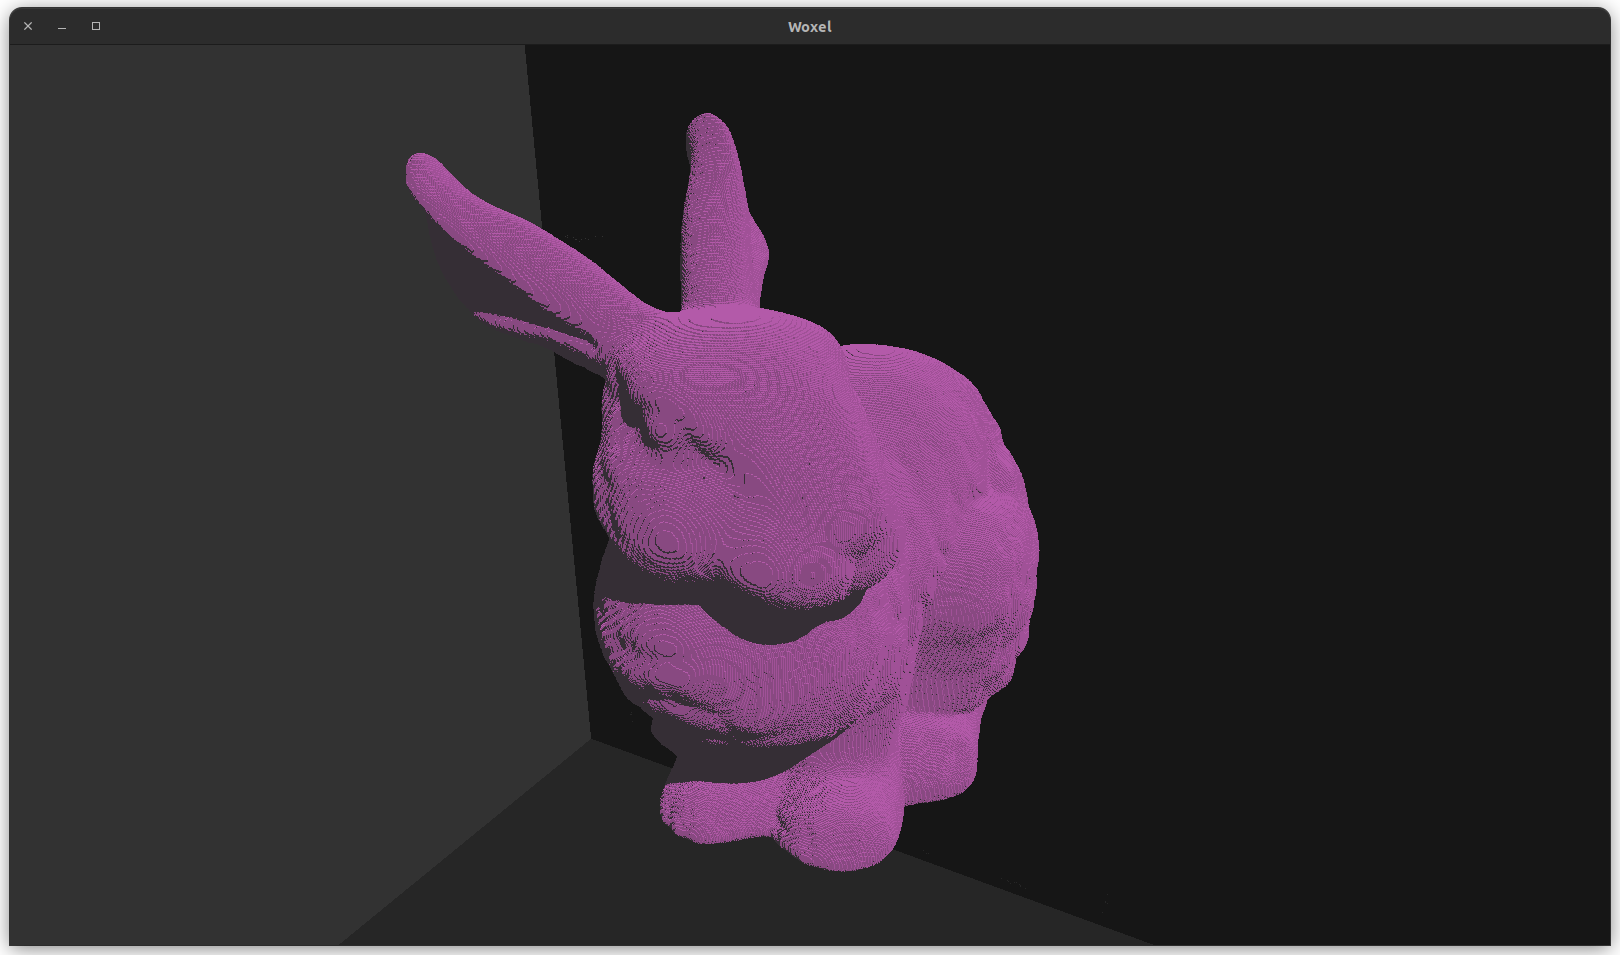
\includegraphics[width=0.8\textwidth]{bunny}
  \caption{Bunny with diffuse pink material, model voxel resolution: $628\times621\times489$}
\end{figure}

\section{Images}

This section shows some images captured in the rendering engine. All the models used are samples from the OpenVDB website\supercite{openvdb:models}. Each of the figures bellow showcase a different functionalities of the engine.

\begin{figure}[H]
  \centering
  \begin{subfigure}[b]{0.48\textwidth}
    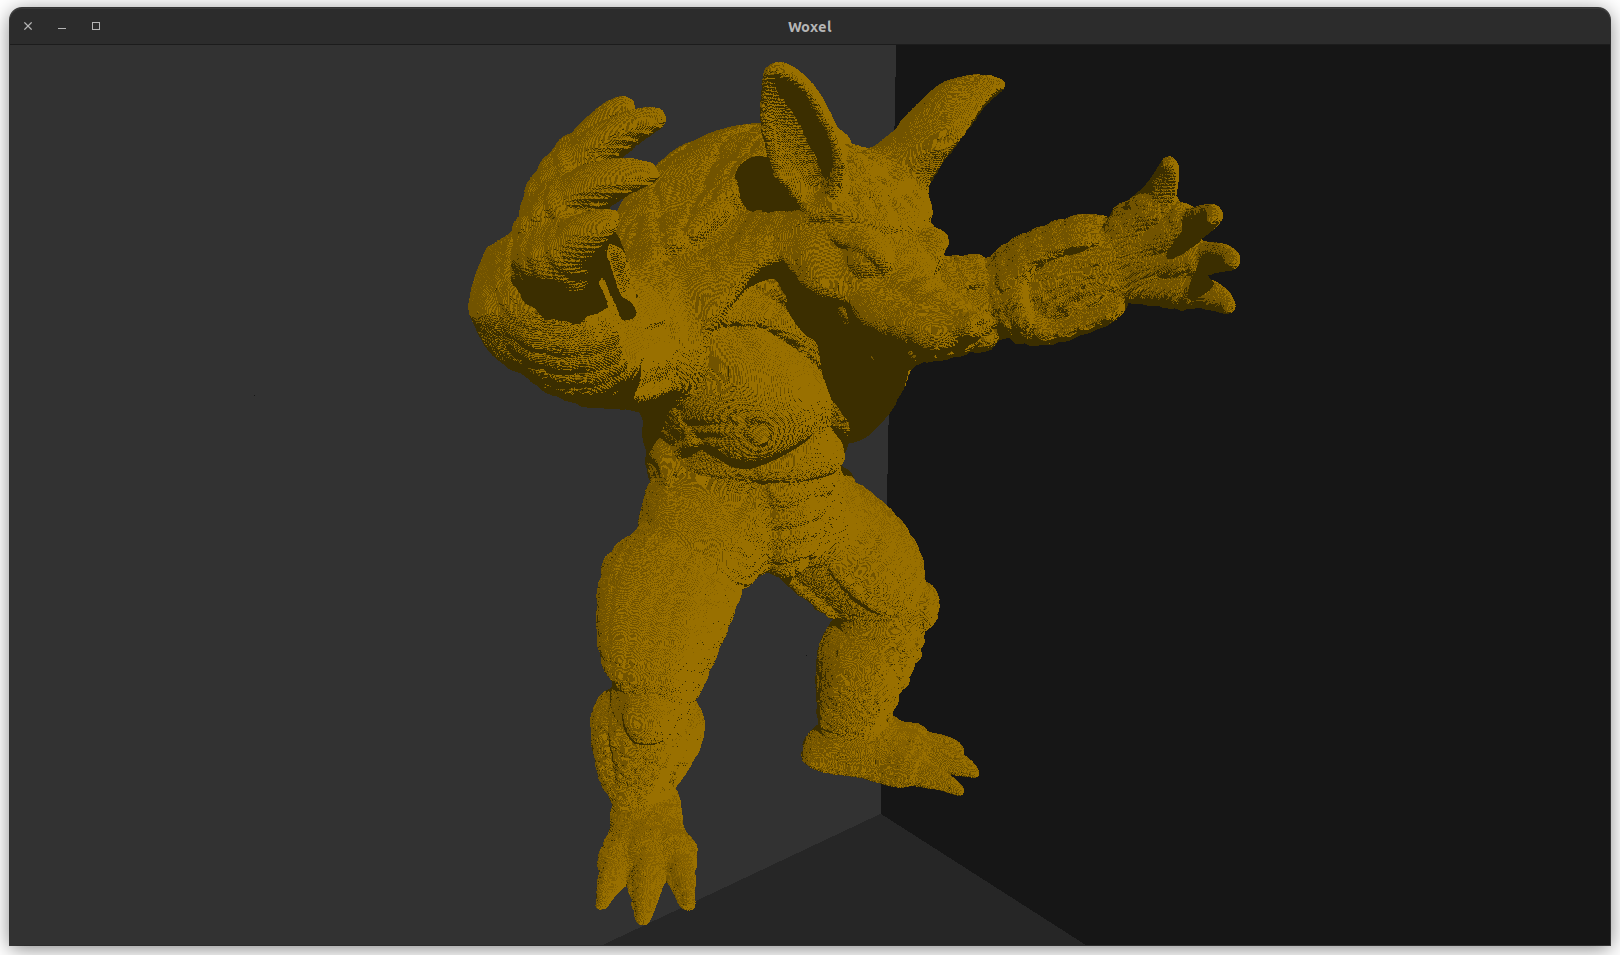
\includegraphics[width=\textwidth]{arm_1}
  \end{subfigure}
  \hfill
  \begin{subfigure}[b]{0.48\textwidth}
    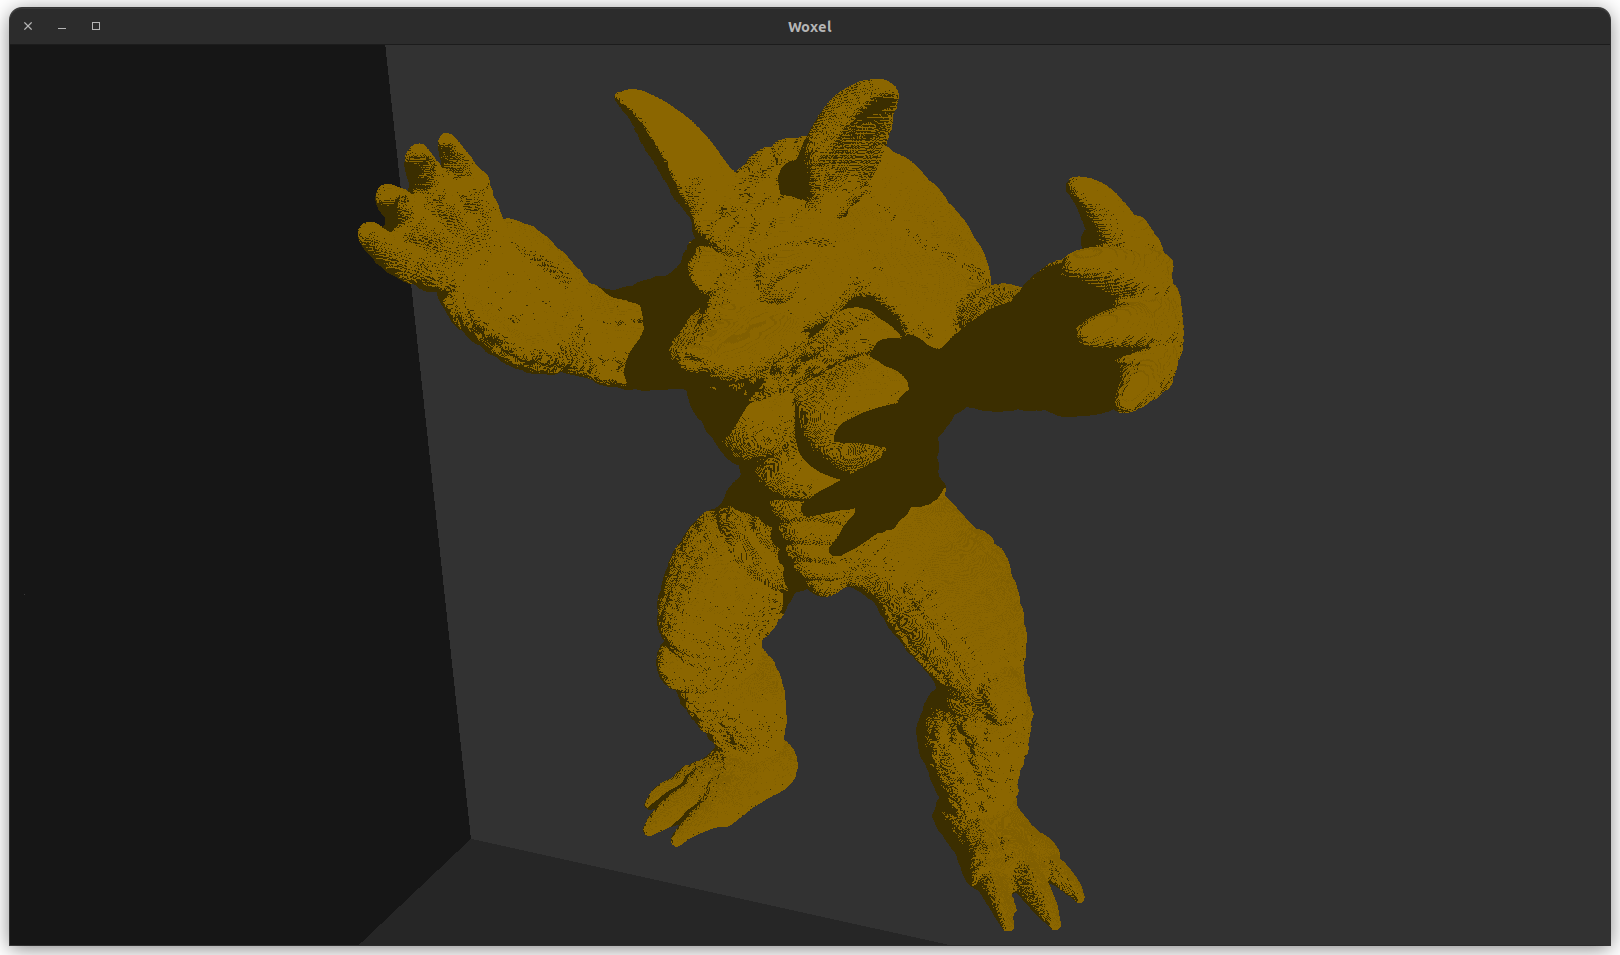
\includegraphics[width=\textwidth]{arm_2}
  \end{subfigure}
  \begin{subfigure}[b]{0.48\textwidth}
    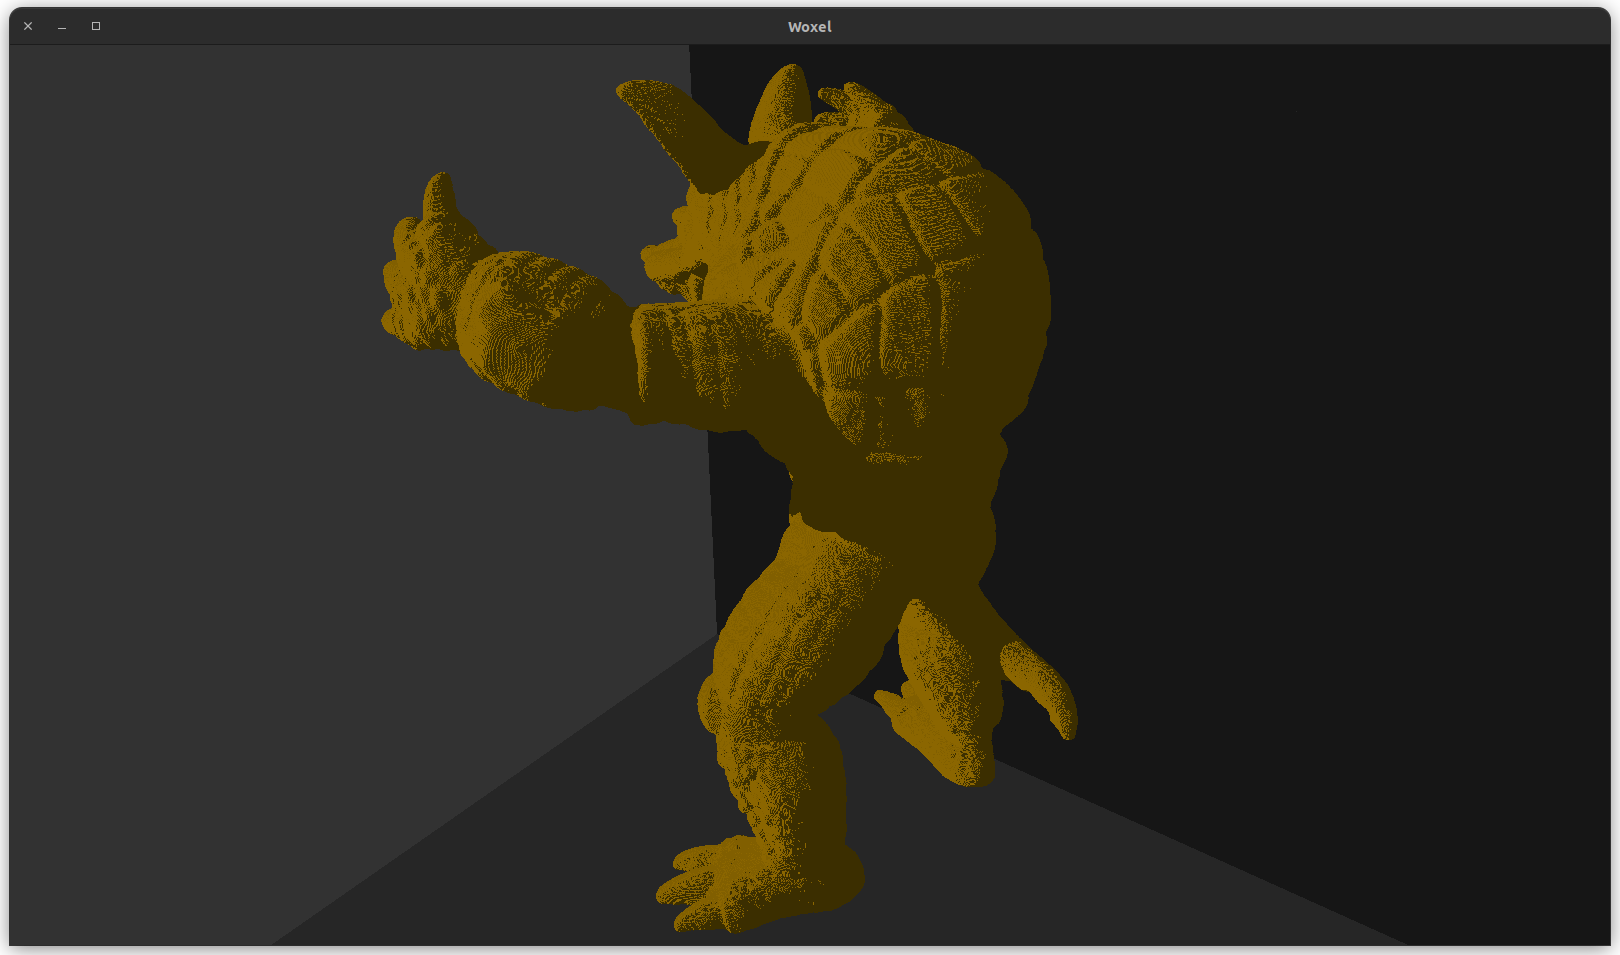
\includegraphics[width=\textwidth]{arm_3}
  \end{subfigure}
  \hfill
  \begin{subfigure}[b]{0.48\textwidth}
    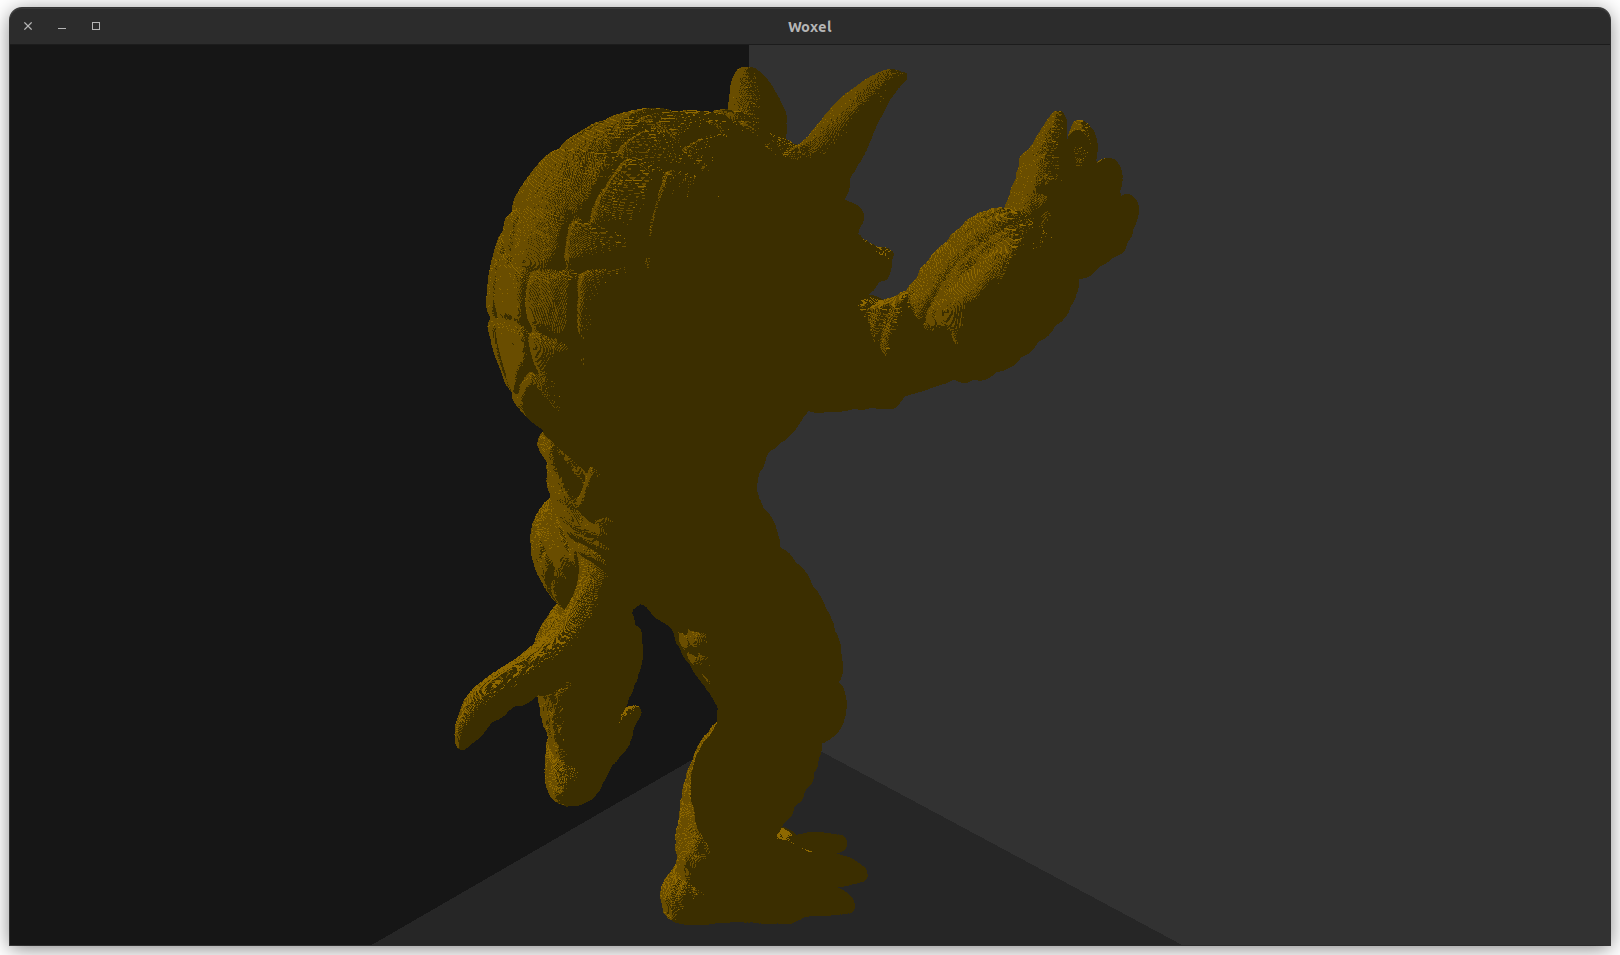
\includegraphics[width=\textwidth]{arm_4}
  \end{subfigure}
  \caption{\textbf{Multiple angles} of an armadilo model with a diffuse material. The voxel resolution of the model is $1276\times1518\times116$}
\end{figure}

\begin{figure}[H]
  \centering
  \begin{subfigure}[b]{0.48\textwidth}
    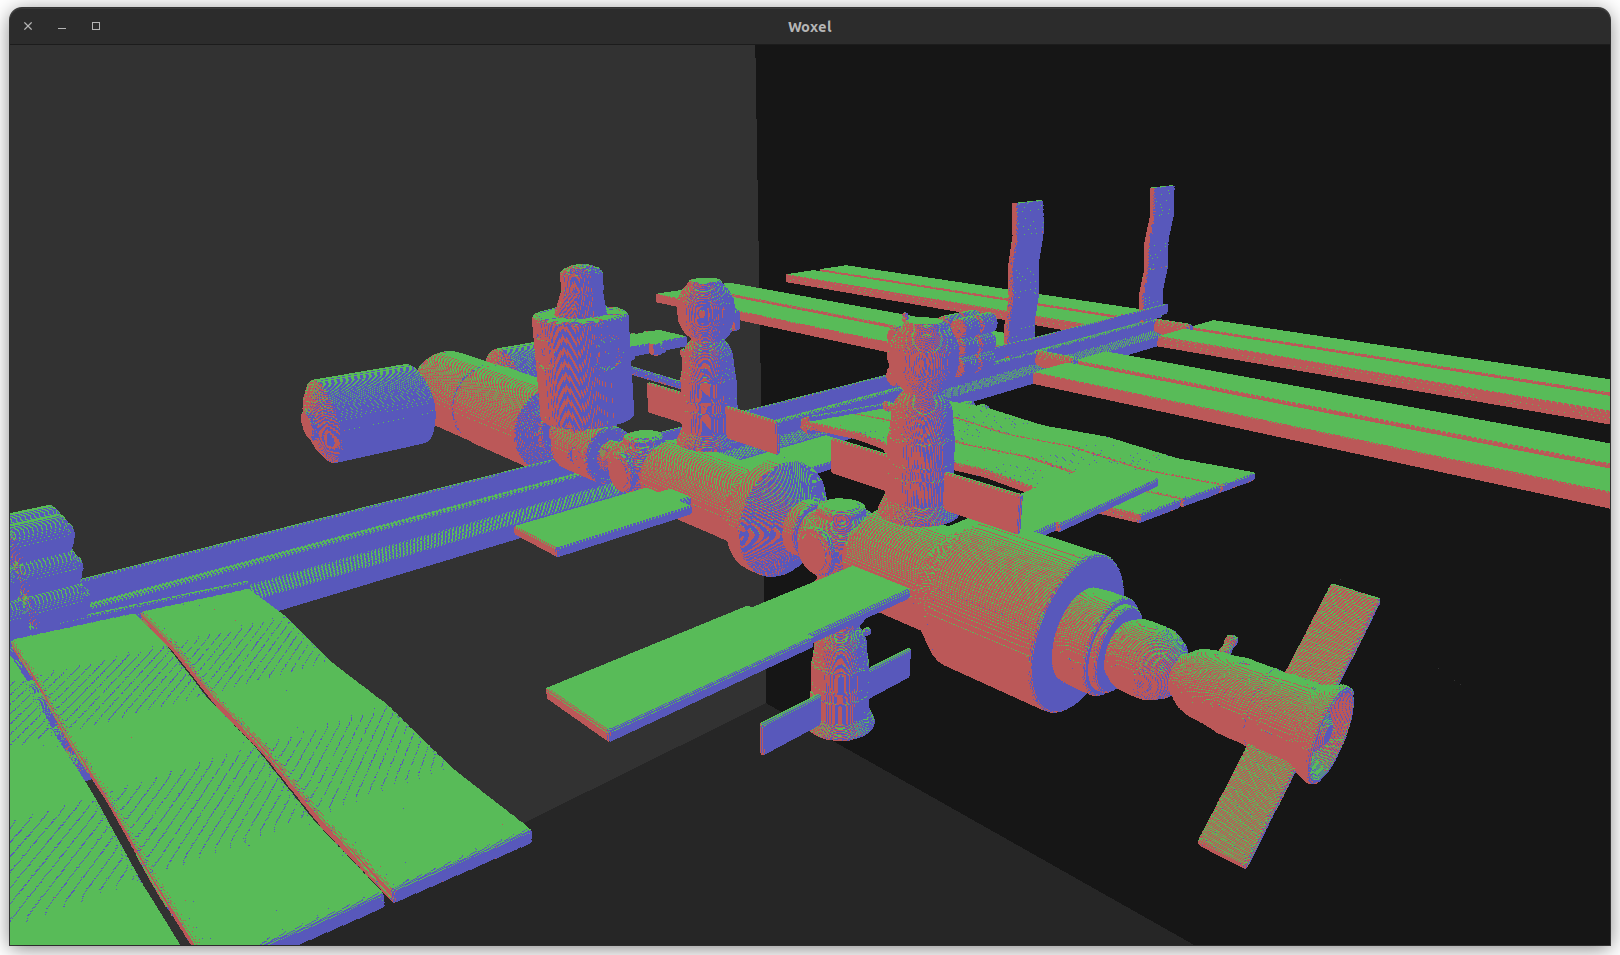
\includegraphics[width=\textwidth]{iss_rgb}
    \caption{RGB}
  \end{subfigure}
  \hfill
  \begin{subfigure}[b]{0.48\textwidth}
    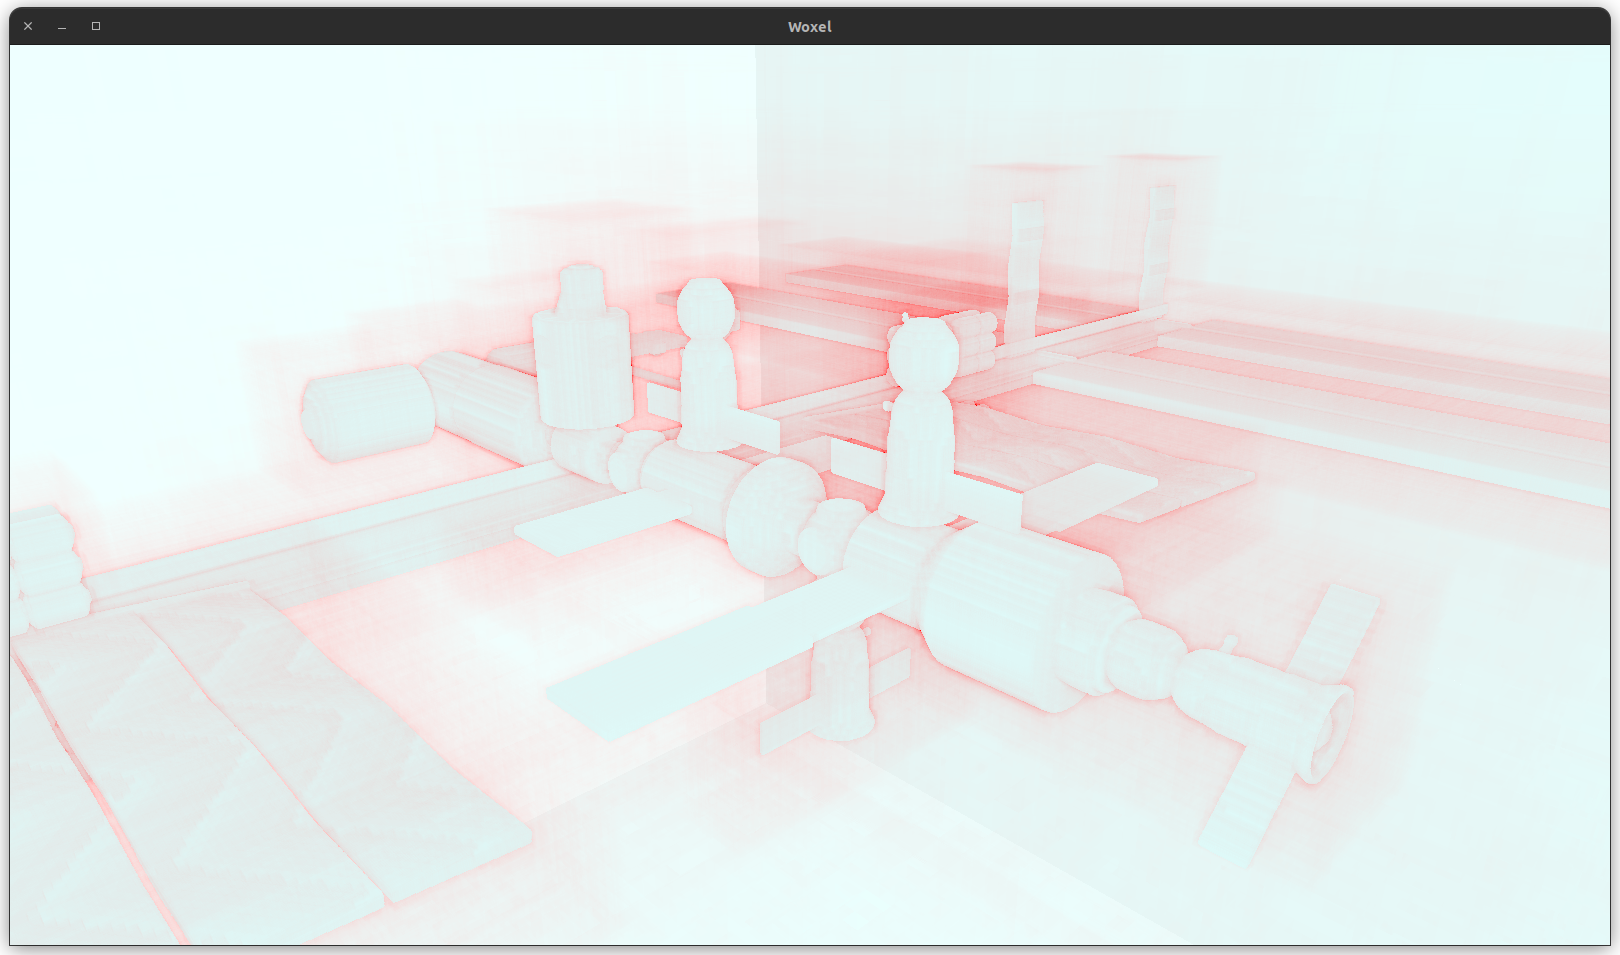
\includegraphics[width=\textwidth]{iss_ray}
    \caption{Ray}
  \end{subfigure}
  \begin{subfigure}[b]{0.48\textwidth}
    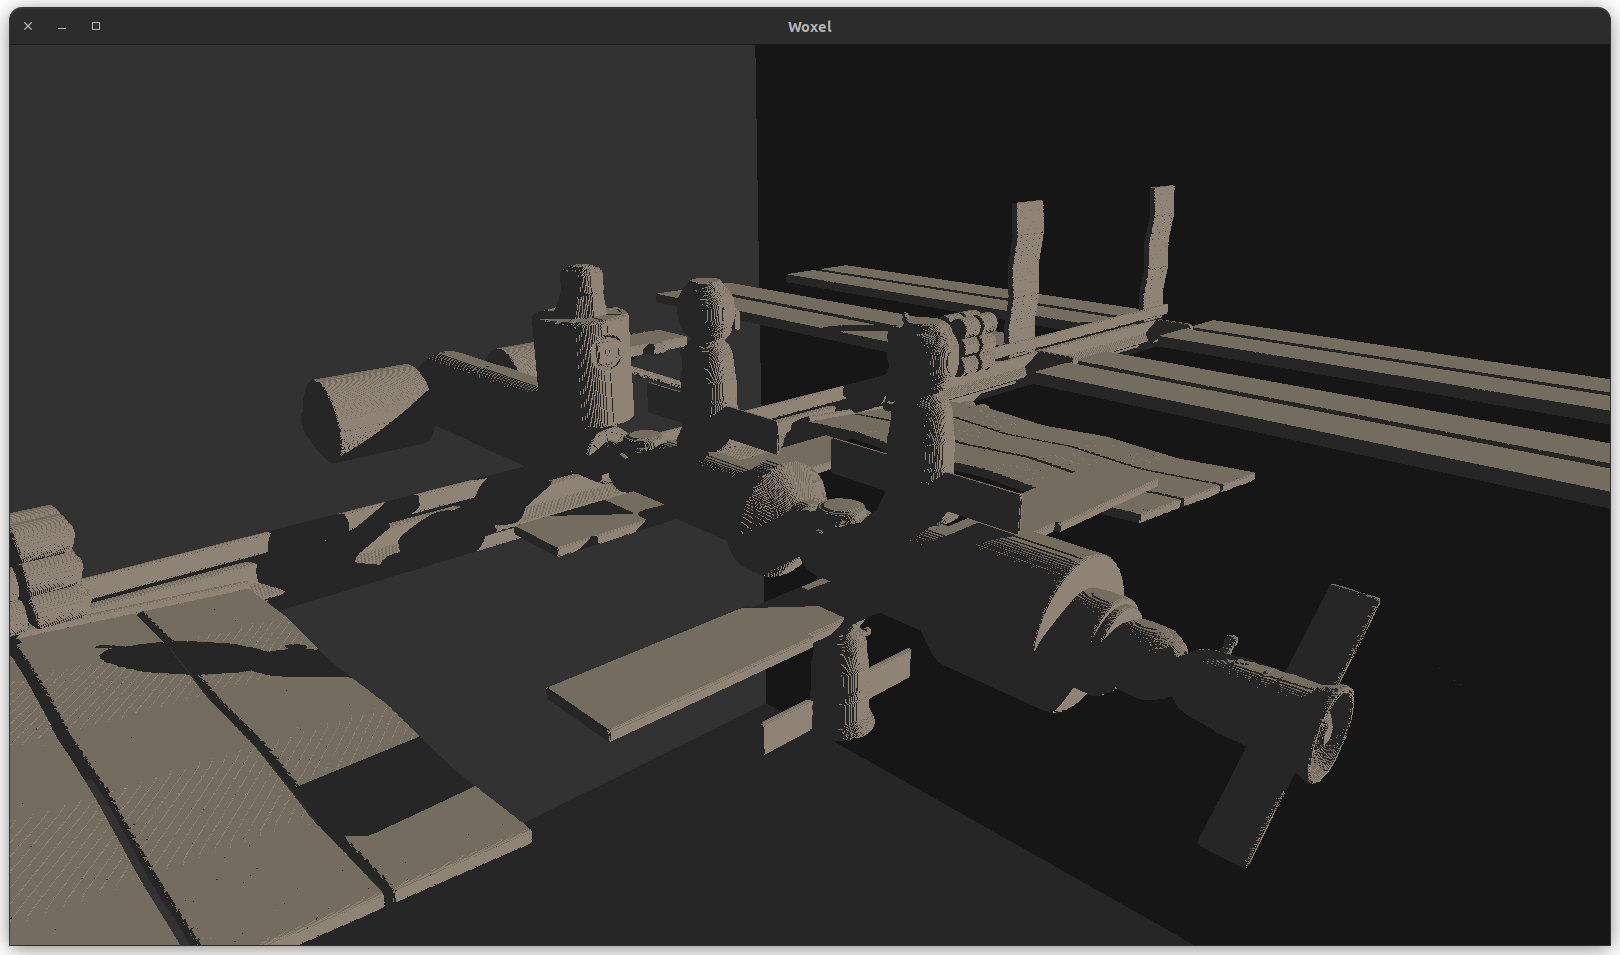
\includegraphics[width=\textwidth]{iss_diffuse}
    \caption{Diffuse}
  \end{subfigure}
  \hfill
  \begin{subfigure}[b]{0.48\textwidth}
    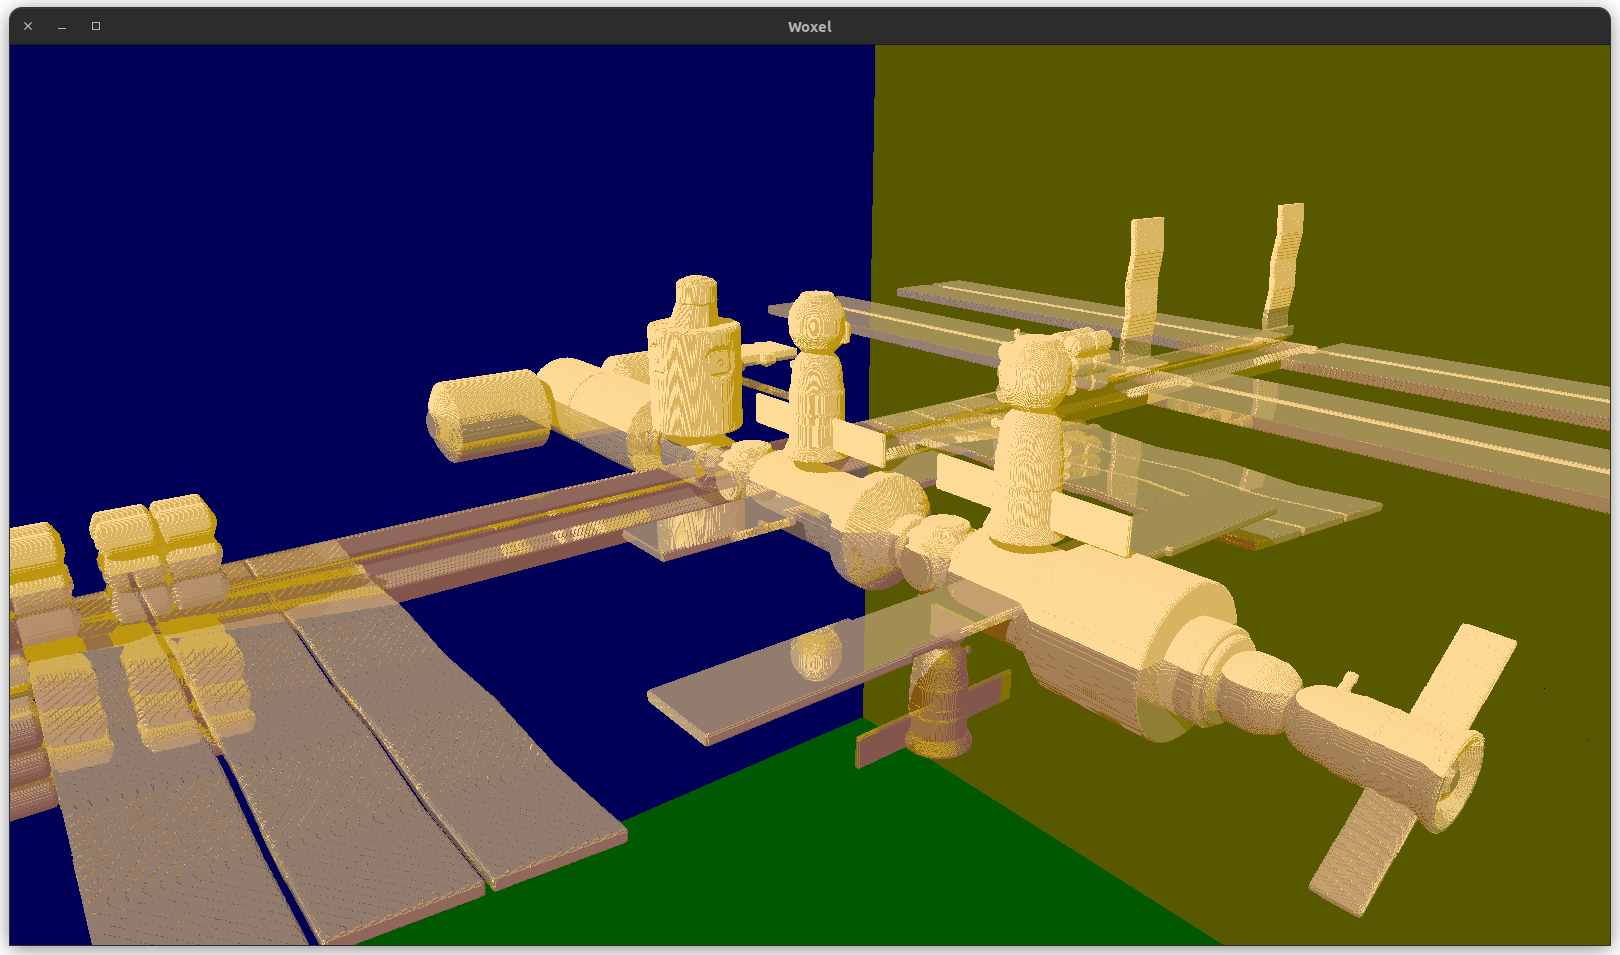
\includegraphics[width=\textwidth]{iss_gloss}
    \caption{Glossy}
  \end{subfigure}
  \caption{\textbf{Render modes} on a ISS model with voxel resolution $4561\times617\times2999$
    (a): RGB mode colors each face based on what axis it is parallel to.
    (b): Ray mode colors each pixel based on how many steps the ray took. The color is interpolated between light blue and red based on how many steps the ray took to go out of bounds or intersect a voxel. Maximum (red) is 200 steps.
    (c): Diffuse mode shows an object with diffuse material lit by sunlight.
    (d): Glossy mode shows a half glossy (bottom), half diffuse (top) model lit by sunlight. The out of bounds box is colored to discriminate which is face reflected on what surface. The reflection of the middle pod with a sphear on top can be seen in the solar panel in the middle. More reflections can be seen in the solar panels one the left and right.
  }
  \label{rendermods}
\end{figure}


\begin{figure}[H]
  \centering
  \begin{subfigure}[b]{0.48\textwidth}
    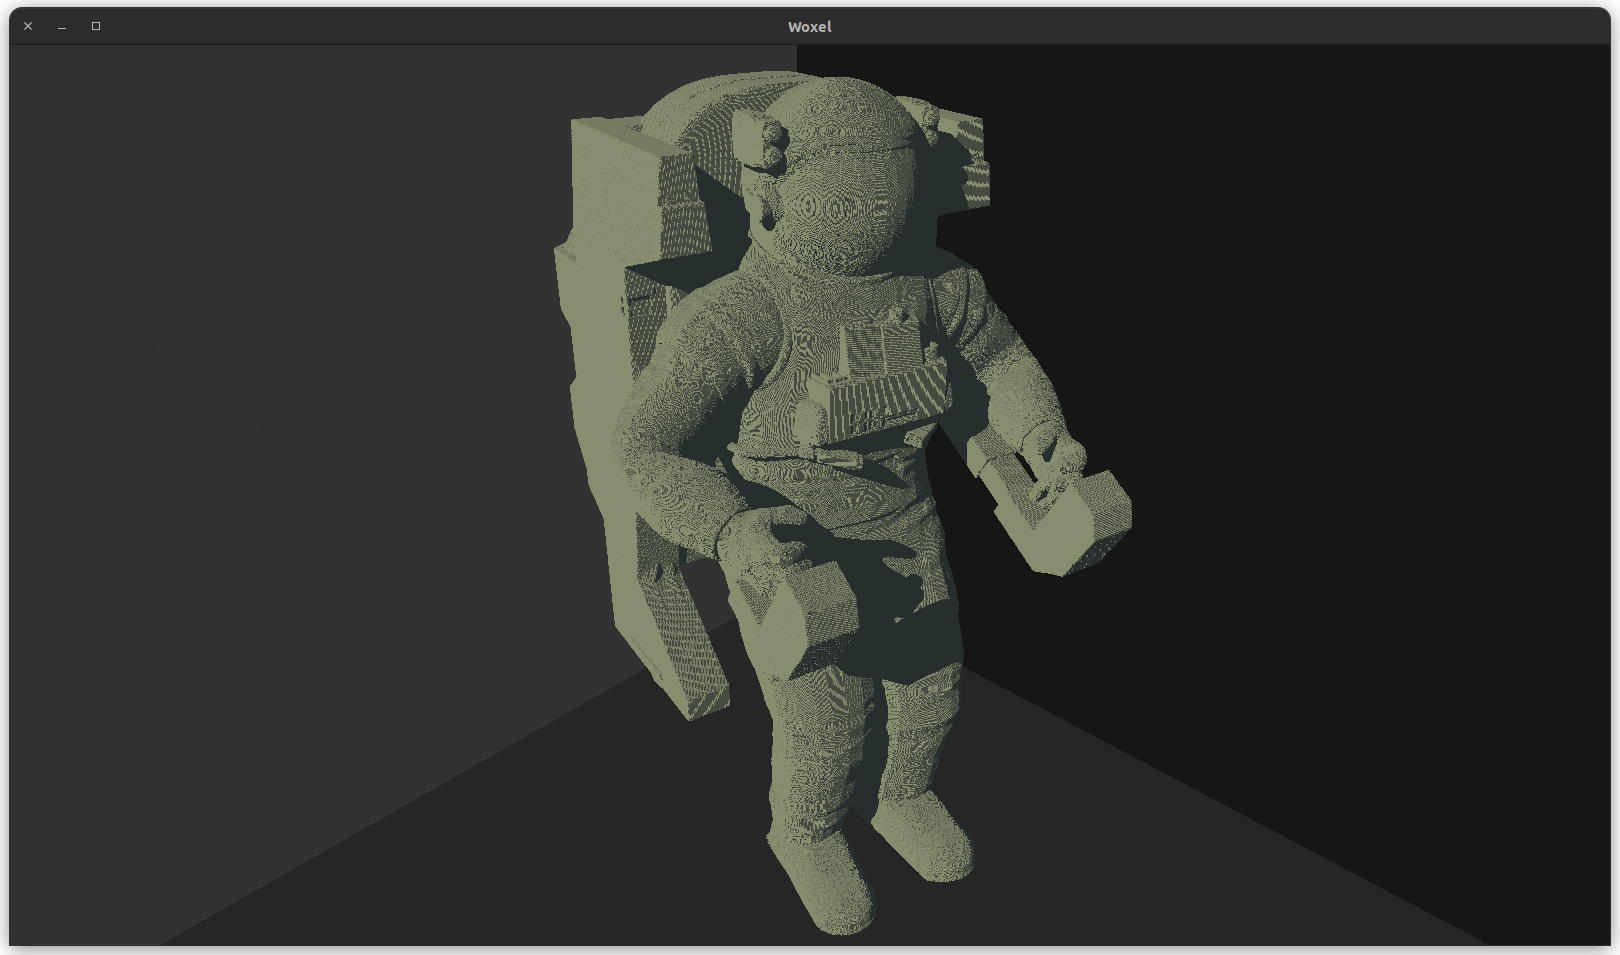
\includegraphics[width=\textwidth]{astro_1}
  \end{subfigure}
  \hfill
  \begin{subfigure}[b]{0.48\textwidth}
    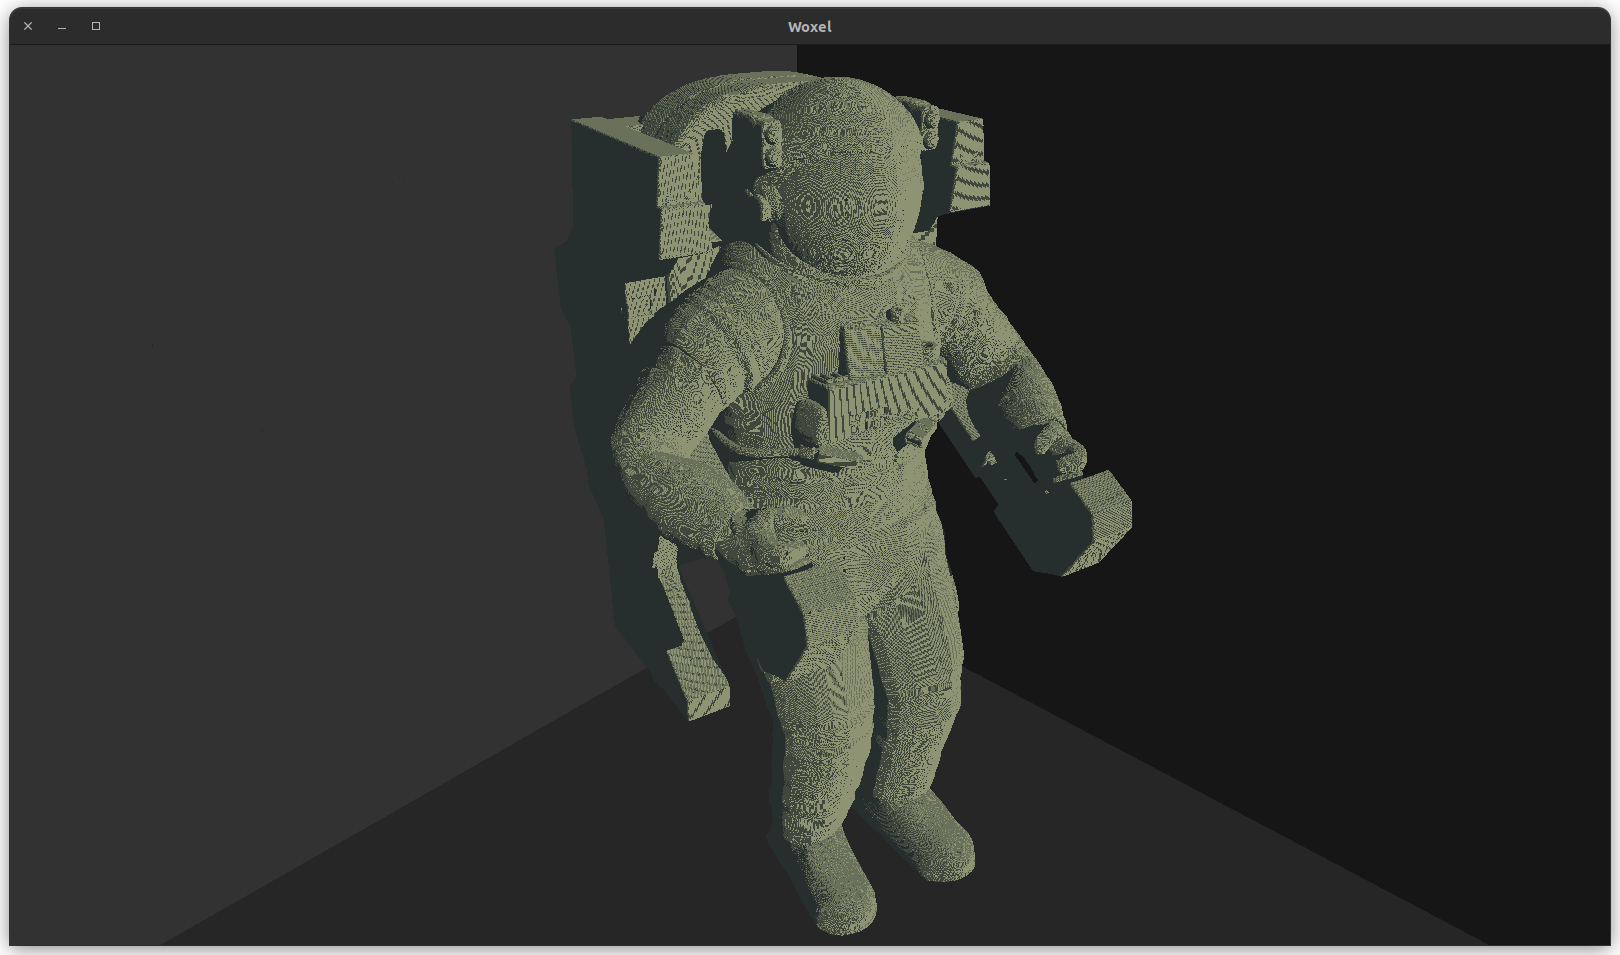
\includegraphics[width=\textwidth]{astro_2}
  \end{subfigure}
  \begin{subfigure}[b]{0.48\textwidth}
    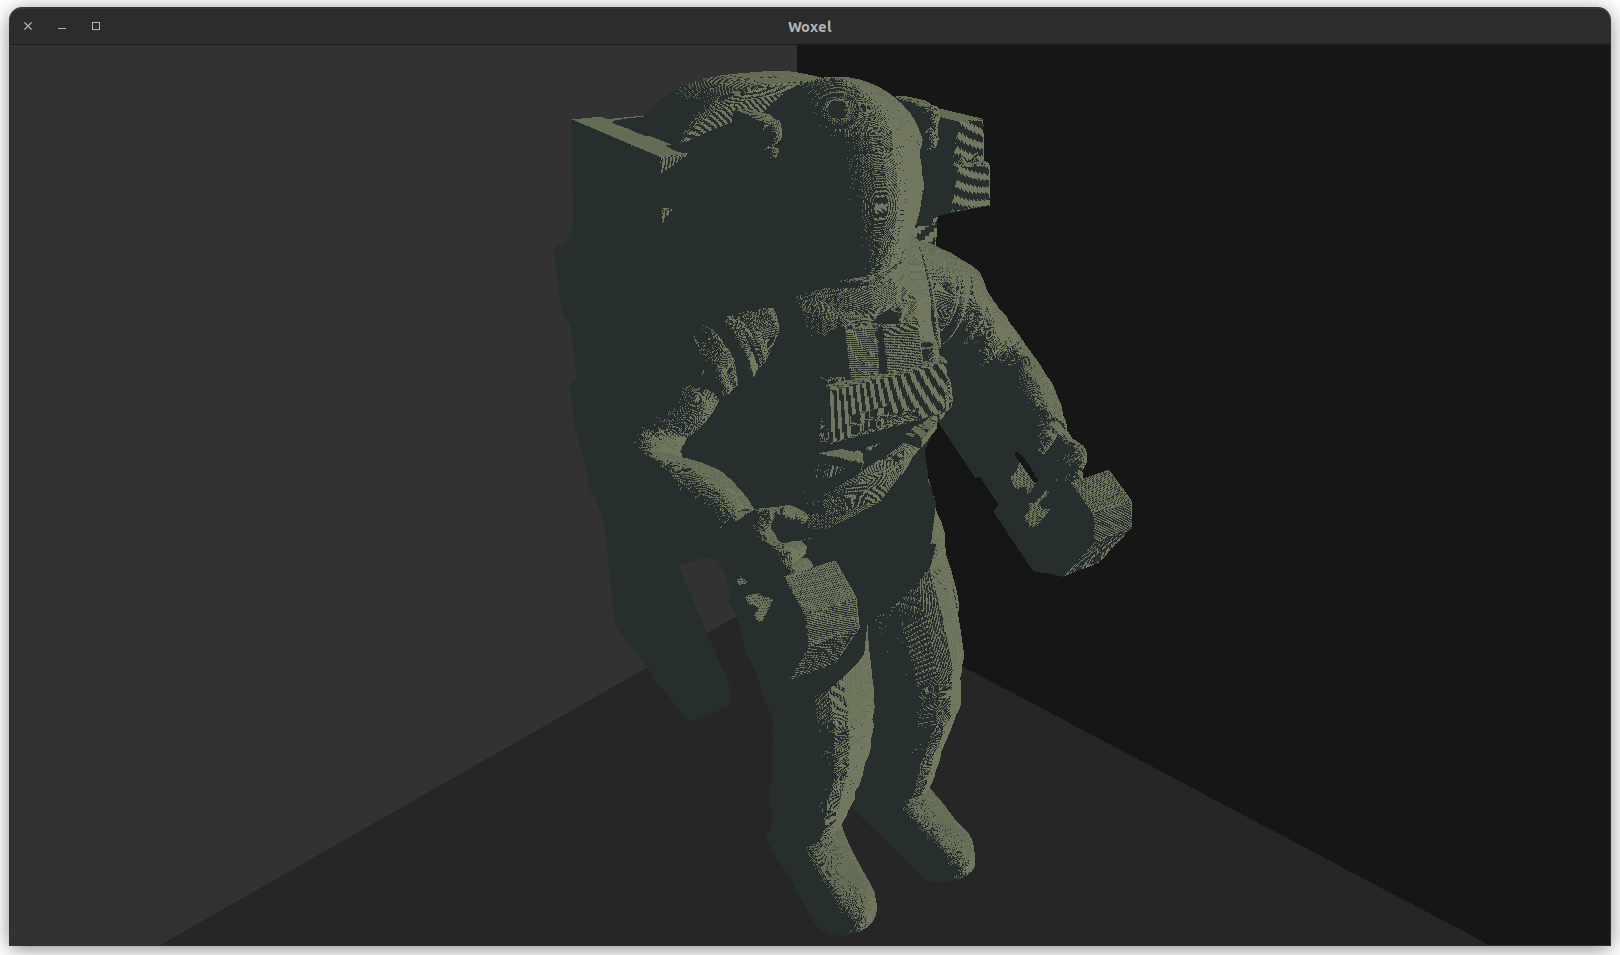
\includegraphics[width=\textwidth]{astro_3}
  \end{subfigure}
  \hfill
  \begin{subfigure}[b]{0.48\textwidth}
    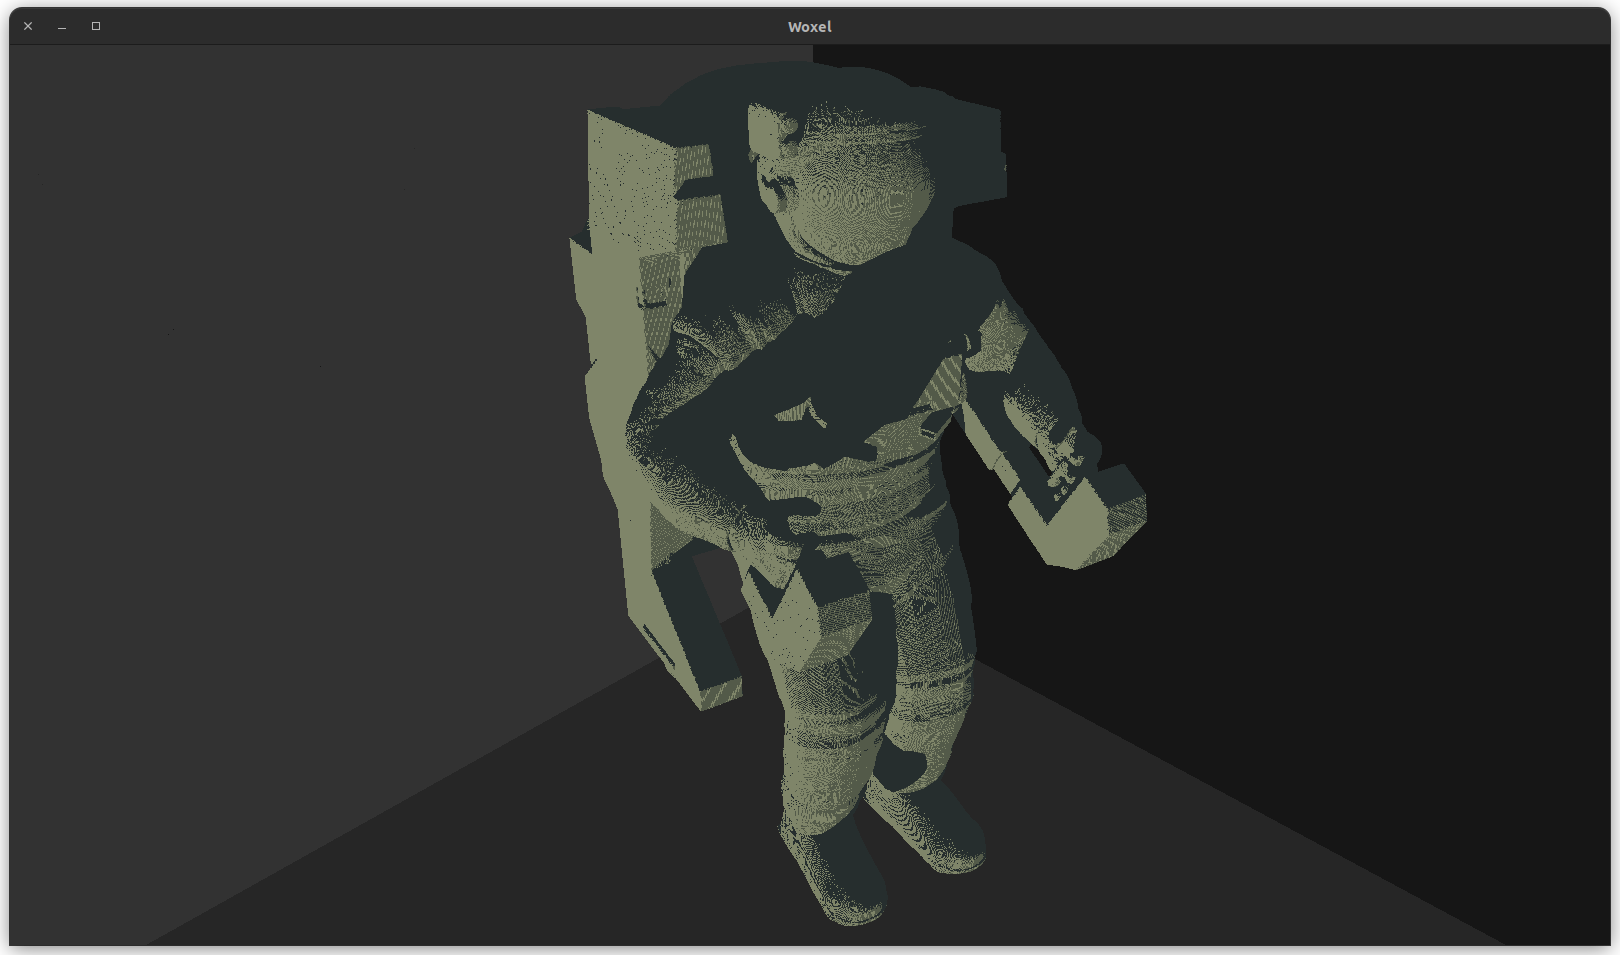
\includegraphics[width=\textwidth]{astro_4}
  \end{subfigure}
  \caption{\textbf{Dynamic Lighting} on an astronaut model. The sunlight is dynmaic, its direction, color and intensity can be changed through the developer GUI in real-time. The voxel resolution of the model is $1481\times2609\times1843$}
\end{figure}

\begin{figure}[H]
  \centering
  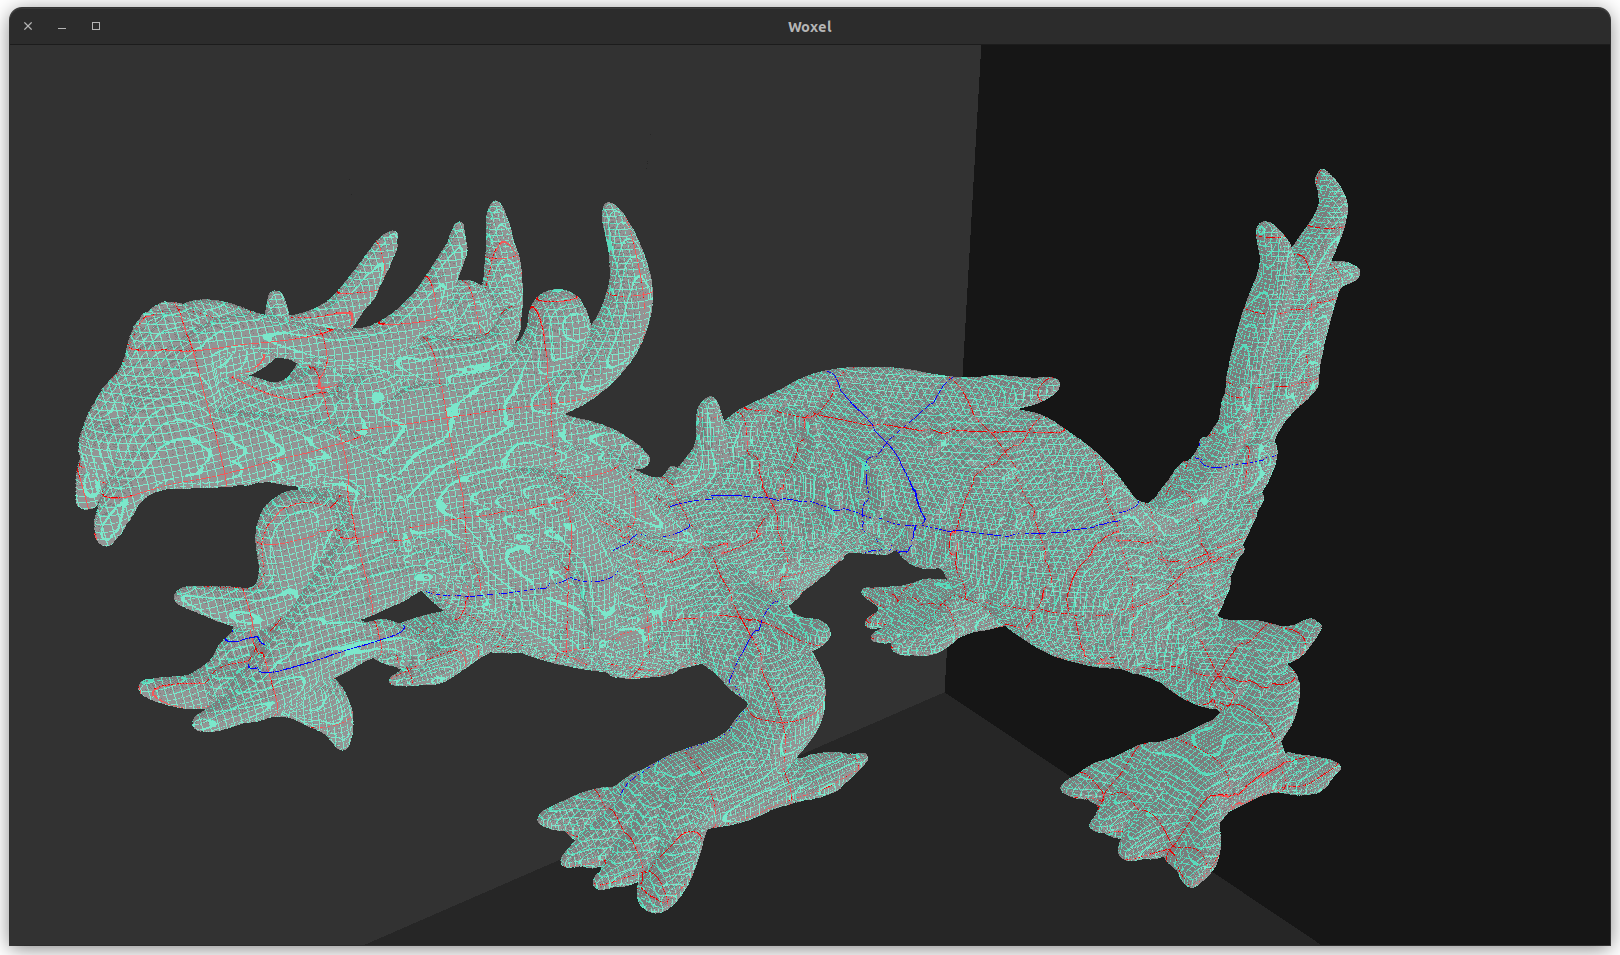
\includegraphics[width=0.8\textwidth]{dragon_3}
  \caption{\textbf{VDB highligthing}: Voxels at the boundries of VDB nodes are highlighted on a dragon model. The grid structure of the VDB can be seen at each level in the hierarchy. Node3, Node4 and Node5 boundries are shown in Cyan, Red and Blue respectively. The voxel resolution of the model is $2023\times911\times1347$}
\end{figure}

\begin{multicols}{2}[]
  \begin{figure}[H]
    \centering
    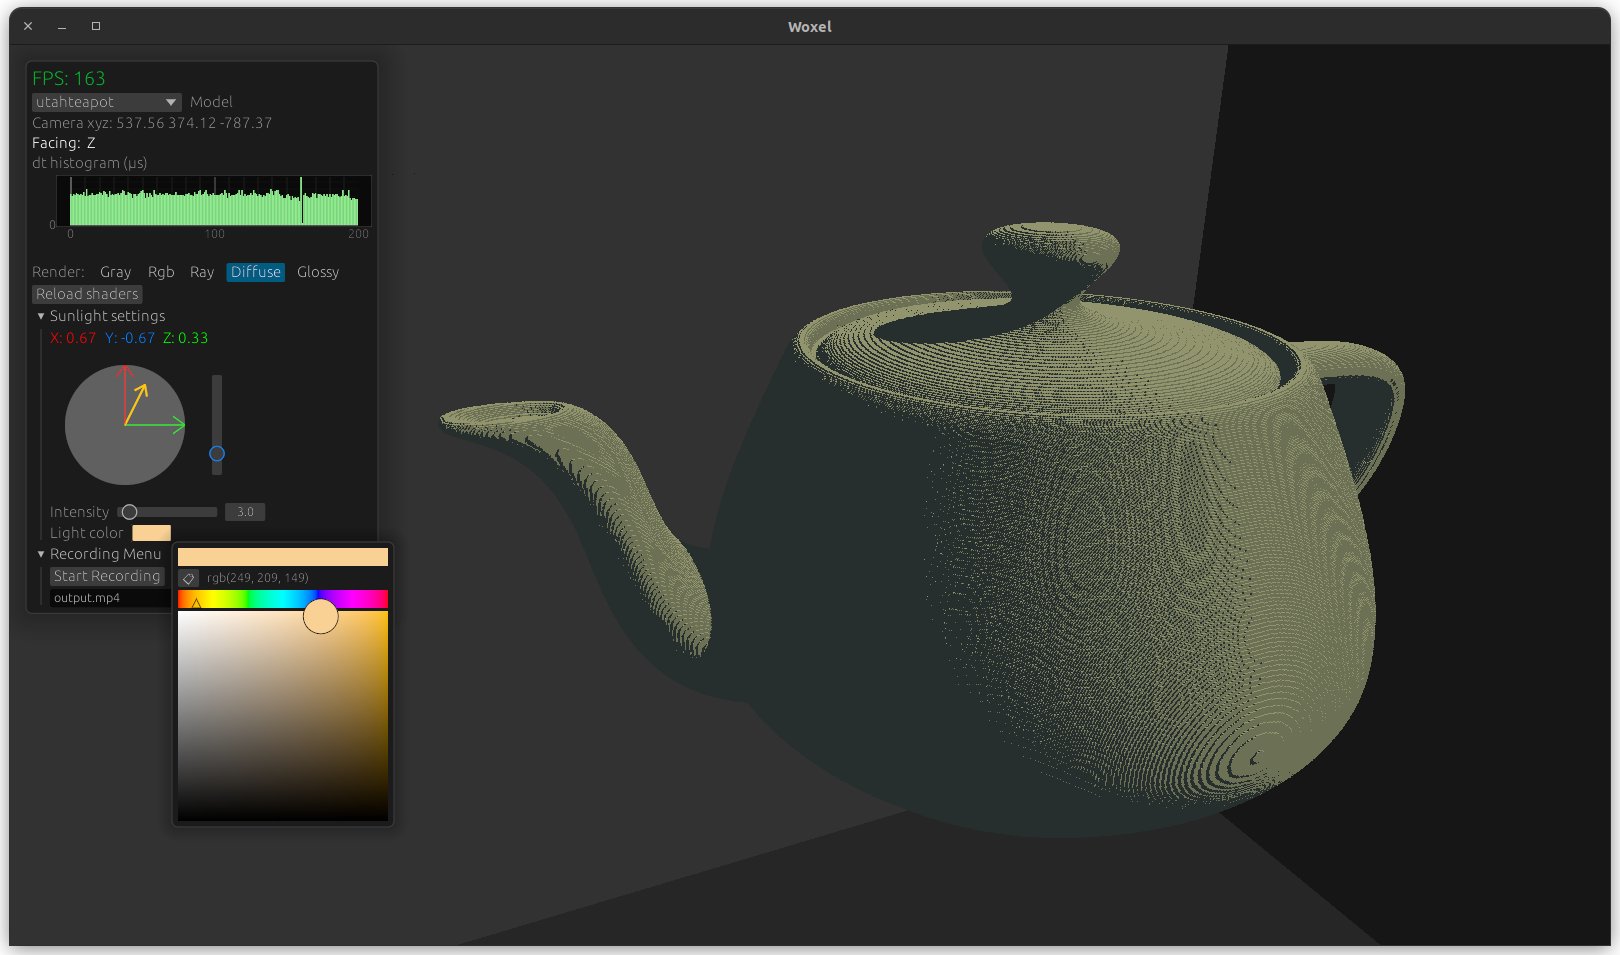
\includegraphics[width=0.96\linewidth]{gui_1}
    \caption{Developer GUI in engine}
  \end{figure}
  The developer GUI has the following uses:
  \begin{enumerate}[itemstep=0mm]
    \item Display current \acrshort{FPS} and histogram of milliseconds per frame.
    \item Changing the model in the viewport through a drop down menu that scans the assets folder for available models.
    \item Camera coordinates and facing direction
    \item Functionality to change between the render modes presented in \cref{rendermods}
    \item The option to reload the shaders while the engine is running.
    \item For the diffuse and glossy render modes there is a sunlight section available.
    \item The recording menu allows setting an output file and starting or ending the recording.
  \end{enumerate}
  \columnbreak
  \begin{figure}[H]
    \centering
    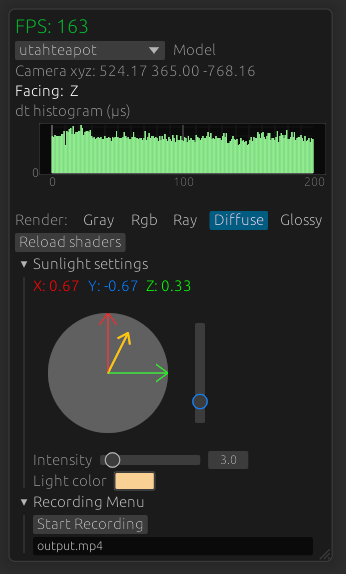
\includegraphics[width=1.0\linewidth]{gui_2}
    \caption{Developer GUI close-up}
    \label{gui}
  \end{figure}
\end{multicols}

\section{Benchmarks}
In this section the ray catsing algorithms are compared against each other on different models and render modes.

The specifications of the machine the experiments where ran on are presented in \cref{specs}.
\begin{table}[h]
  \centering
\begin{tabular}{|c||c|}
  \hline
  \multicolumn{2}{|c|}{Experiment machine specifications} \\
  \hline
  OS & Ubuntu 22.04.3 LTS x86\_64\\
  \hline
  CPU & AMD Ryzen 7 5800H with Radeon\\
  \hline
  GPU &  NVIDIA GeForce RTX 3070 Mobile\\
  \hline
  RAM & 8192MiB \\
  \hline
  FMA & Enabled \\
  \hline
\end{tabular}
  \caption{Experiment machine specifications}
  \label{specs}
\end{table}

\subsection{Comparing DDA, HDDA and HDDA+SDF}

First the average millseconds per frame are compared for the DDA, HDDA and HDDA+SDF algorithms is compared on the teapot model at 3 distinct distances from the model, one further a way, ore closer and one near the model.

\begin{table}[h]
  \centering
  \begin{tabular}{|c||c|c|c|}
    \hline
    & 2000m & 1000m & 500m \\
    \hline
    DDA & 100ms* & 100ms* & 50ms \\
    \hline
    HDDA & 9.4ms & 12.5ms & 14.4ms \\
    \hline
    HDDA & 9.4ms & 12.5ms & 14.4ms \\
    \hline
    HDDA+SDF & 6ms** & 6.4ms & 7.6ms\\
    \hline
  \end{tabular}
  \caption{Milliseconds per frame of rendering the teapot model using DDA, HDDA, HDDA+SDF at far, medium, and close distance. A voxel is considered $1\rm{m}\times1\rm{m}\time1\rm{m}$. (*): Model doesn't show in viewport because the algoirhtm exceeds the maximum step size. This time can be treated as the wors-case scenario, casting bouncing the maximum number of times for each pixel. (**): Frame rate cap is hit at 165 FPS}
\end{table}

\section{Future work}
\section{Final remarks}

\include{chapters/conclusion.tex}

%%%%%%%%%%%%%%%%%% REFERRENCES %%%%%%%%%%%%%%%%%%
\printbibliography[title={References},heading=bibintoc]


%%%%%%%%%%%%%%%%%% ACRONYMS %%%%%%%%%%%%%%%%%%
\newpage
\printglossary[type=\acronymtype]

\end{document}
